\documentclass[tikz,border=10pt]{standalone}
% no extra libraries needed
\begin{document}
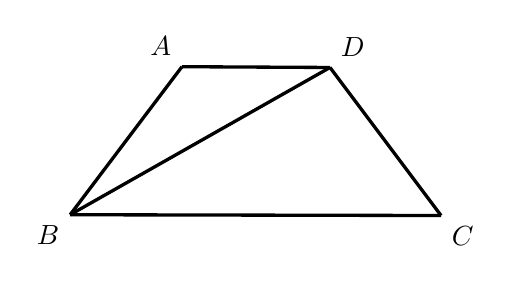
\begin{tikzpicture}[line width=1.2pt, line join=round]
  % vertices (pixel coords, y flipped, scale 1/100)
  \coordinate (A) at (2.12,-0.65);
  \coordinate (B) at (0.70,-2.53);
  \coordinate (C) at (5.41,-2.54);
  \coordinate (D) at (4.00,-0.66);

  % quadrilateral edges
  \draw (A) -- (B);
  \draw (B) -- (C);
  \draw (C) -- (D);
  \draw (D) -- (A);

  % interior diagonal BD (no AC)
  \draw (B) -- (D);

  % labels outside the vertices
  \node[above left] at (A) {$A$};
  \node[above right] at (D) {$D$};
  \node[below left] at (B) {$B$};
  \node[below right] at (C) {$C$};
\end{tikzpicture}
\end{document}